% 行列投影迭代法：Kaczmarz、扩展Kaczmarz与停止检验
\section{行列投影迭代法}
\label{sec:ls-row-projection}

前两节的迭代每轮都要访问整个矩阵。数据按行陆续到达或只方便逐行读取时，可以每次只让一个方程成立，用投影逐步求解。标准Kaczmarz算法处理相容方程；方程不相容时，再用列投影修正右端，形成扩展Kaczmarz算法。本节$\bm A\in\mathbb R^{m\times d}$不必是方阵，两种算法都以$\bm A,\bm b$为输入、以$\bm x$为输出，投影中的残差和辅助向量只是内部状态。

\subsection{Kaczmarz算法}
\label{sec:ls-kaczmarz}

\subsubsection{主要思想}

Kaczmarz算法（Kaczmarz method）把当前解正交投影到某一个行方程的超平面上。记第$i$行为$\bm a_i^\top$，非零行的方程$\bm a_i^\top\bm x=b_i$的解集是以$\bm a_i$为法向量的超平面；由正交投影（第~\ref{sec:ls-orthogonal-projection}节），离$\bm x_k$最近的点沿法向得到，把它写成$\bm x_k+t\bm a_i$代入方程，即得修正方向$\bm a_i$和修正长度$t=(b_i-\bm a_i^\top\bm x_k)/\lVert\bm a_i\rVert_2^2$。一次更新让所选方程成立，却可能改变其他行的残差；方程相容时各超平面有公共点，反复投影便逐渐逼近它。本小节假设方程相容，只遍历非零行。

\subsubsection{算法实现}

\paragraph{初始化}
超参数单独列出：初值$\bm x_0$，固定的循环访问顺序，残差容差$\mathrm{atol},\mathrm{rtol}$，以及最大更新次数$K$；要求最小范数解时取$\bm x_0=\bm 0$。内部保存当前解$\bm x_k$和当前行的修正量$\bm\delta_k$，全局残差只在初始时和每轮完整扫掠后计算。初始化计数$k=0$，若$K=0$则直接取$\bm x=\bm x_0$并结束。

\paragraph{行投影}
之后按循环顺序选出行$i_k$，计算
\[
\bm\delta_k=\frac{b_{i_k}-\bm a_{i_k}^\top\bm x_k}{\lVert\bm a_{i_k}\rVert_2^2}\,\bm a_{i_k},\qquad
\bm x_{k+1}=\bm x_k+\bm\delta_k ,
\]
每完成一次行更新便把$k$加一。

\paragraph{停止检查}
达到更新次数上限时立即结束并取当前$\bm x$，即使这一轮尚未扫完；在初始时和每轮完整扫掠后，若原残差$\lVert\bm b-\bm A\bm x_k\rVert_2$不超过第~\ref{sec:ls-matrix-splitting}节的阈值$\mathrm{atol}+\mathrm{rtol}\lVert\bm b\rVert_2$，也结束并取当前$\bm x$。

\paragraph{随机选行}
随机版本只把选行规则改为按概率$p_i=\lVert\bm a_i\rVert_2^2/\lVert\bm A\rVert_F^2$独立抽样，投影公式不变，每次更新后检查全局残差和次数上限。零行的概率为零，不会被抽到，也就不会出现除以零。

\begin{example}[Kaczmarz算法的前两步]
\label{ex:ls-kaczmarz-two-steps}
用例~\ref{ex:ls-stationary-running-example}的方程，行$\bm a_1=(4,1)^\top$，$\bm a_2=(1,3)^\top$，平方范数分别为$17$和$10$，从$\bm x_0=\bm 0$出发按$1,2$的顺序投影。第一步第一行的残差为$1-0=1$，修正长度$t=1/17$，得$\bm x_1=(4/17,\,1/17)^\top$，此时$4x_1+x_2=1$成立。第二步第二行的残差为$2-(4/17+3/17)=27/17$，修正长度$t=27/170$，得$\bm x_2=(4/17,1/17)^\top+\tfrac{27}{170}(1,3)^\top=(67/170,\,91/170)^\top$，第二个方程成立，第一个方程又不再成立。到$\bm x_\star=(1/11,7/11)^\top$的距离依次约为$0.643$、$0.595$、$0.320$。
\end{example}

\subsubsection{算法分析}

\paragraph{收敛性}
循环版本的收敛可以由投影的几何性质直接得到。下面$\bm A^\dagger$为伪逆（第~\ref{sec:ls-pseudoinverse}节），$\bm I-\bm A^\dagger\bm A$是到零空间$\mathcal N(\bm A)$的正交投影。
\begin{theorem}[相容方程上循环Kaczmarz的收敛]
\label{thm:ls-kaczmarz-convergence}
设$\bm A\bm x=\bm b$相容且$\bm A\neq\bm 0$，令$\bm x_\star=\bm A^\dagger\bm b+(\bm I-\bm A^\dagger\bm A)\bm x_0$。按固定循环顺序遍历非零行时，$\bm x_\star$是方程的解，到它的距离逐步不增，且每完成一轮按与初值无关的因子$q<1$几何收缩，从而$\bm x_k\to\bm x_\star$。特别地，$\bm x_0=\bm 0$时极限是最小范数解$\bm A^\dagger\bm b$。
\end{theorem}
\begin{proof}
对任一解$\bm y$，由$\bm a_i^\top\bm y=b_i$，更新可写成$\bm x_{k+1}-\bm y=\bm P_i(\bm x_k-\bm y)$，其中$\bm P_i=\bm I-\bm a_i\bm a_i^\top/\lVert\bm a_i\rVert_2^2$是到$\bm a_i^\perp$的正交投影，由勾股关系
\[
\lVert\bm x_{k+1}-\bm y\rVert_2^2=\lVert\bm x_k-\bm y\rVert_2^2-\frac{\bigl(\bm a_i^\top(\bm x_k-\bm y)\bigr)^2}{\lVert\bm a_i\rVert_2^2}.
\]
每次修正都是某个$\bm a_i$的倍数，留在行空间$\mathcal R(\bm A^\top)$中，所以$\bm x_k$的零空间分量始终等于$\bm x_0$的零空间分量；$\bm A\bm x_\star=\bm A\bm A^\dagger\bm b=\bm b$，且误差$\bm\varepsilon_k=\bm x_k-\bm x_\star$始终在行空间中。一轮的误差映射是固定的$\bm K=\bm P_{i_p}\cdots\bm P_{i_1}$，各$\bm P_i$都把行空间映到自身。若行空间中的$\bm v$满足$\lVert\bm K\bm v\rVert_2=\lVert\bm v\rVert_2$，由上式每次投影都没有缩短长度，$\bm v$依次与每个非零行正交，于是$\bm v\in\mathcal N(\bm A)\cap\mathcal R(\bm A^\top)=\{\bm 0\}$。取行空间的标准正交基排成$\bm Q$，则$\bm C=\bm Q^\top\bm K\bm Q$使$\bm I-\bm C^\top\bm C$正定；由Rayleigh--Ritz定理（定理~\ref{thm:matrix-analysis-rayleigh-ritz}），其最小特征值$\mu\in(0,1]$，所以$\lVert\bm C\rVert_2\leq q=\sqrt{1-\mu}<1$。由第~\ref{sec:ls-convergence}节的固定更新结论，轮末误差几何地趋于零，轮内距离又不增，整个序列收敛到$\bm x_\star$。
\end{proof}
零初值使迭代始终留在行空间中，相容而解不唯一时选出最小范数解；任意初值的极限同样满足方程，但带着初值的零空间分量。

\paragraph{收敛速度与代价}
收敛速度受各行之间的夹角和访问顺序影响：行越接近两两正交，一轮去掉的误差越多。图~\ref{fig:ls-kaczmarz-projection-path}画出了例~\ref{ex:ls-kaczmarz-two-steps}的路径。二维时，第一步之后误差已经平行于刚投影过的直线，此后每次投影都把误差长度乘以两条直线法向夹角的余弦$|\bm a_1^\top\bm a_2|/(\lVert\bm a_1\rVert_2\lVert\bm a_2\rVert_2)=7/\sqrt{170}\approx0.537$；例中距离从$0.595$降到$0.320$，比值正是这个数。两条直线越接近垂直，余弦越小，折线收拢得越快；越接近平行，路径就在狭窄的夹角里来回往复。一次投影的成本为$O(\operatorname{nnz}(\bm a_i))$，全局残差检查另需一次完整的矩阵乘向量。

\begin{figure}[htbp]
  \centering
  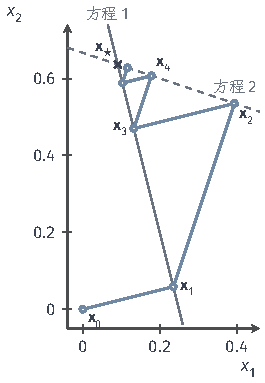
\includegraphics[width=44.81mm]{figures/01-basic-mathematics/03-vectors-matrices-and-multivariate-functions/tikz/c5-kaczmarz-projection-path/figure.pdf}
  \caption{循环Kaczmarz在贯穿例上的交替投影路径。实线为第一个方程$4x_1+x_2=1$的解集，虚线为第二个方程$x_1+3x_2=2$的解集；从$\bm x_0=\bm 0$出发依次垂直投影到两条直线上，折线连接精确计算的前六个迭代点并逐步收拢到交点$\bm x_\star$，图中标出前四个。坐标轴等比例，投影段与对应直线垂直。}
  \label{fig:ls-kaczmarz-projection-path}
\end{figure}

\paragraph{随机版本与不相容情形}
随机选行的概率收敛及其速率由Strohmer与Vershynin给出\scite{math-strohmer2009randomized}，证明要用到期望，留到第~\ref{chap:random-variables}章建立概率基础之后。不相容时情况不同。取$\bm A=(1,1)^\top$，$\bm b=(0,1)^\top$，未知量是标量，两行分别要求$x=0$和$x=1$；两行长度都为一，投影化为$x\gets b_i$，循环投影便在$0$与$1$之间往返，而最小二乘解是$\hat x=1/2$。随机选行时每一步$x$也只取$0$或$1$，所以仅改选行方式不能保证得到最小二乘解。不相容问题交给下一个算法处理。

\subsection{扩展Kaczmarz算法}
\label{sec:ls-extended-kaczmarz}

\subsubsection{主要思想}

不相容的根源在右端：把$\bm b$分解为$\bm b_\parallel+\bm b_\perp$，$\bm b_\parallel\in\mathcal R(\bm A)$，$\bm b_\perp\in\mathcal N(\bm A^\top)$，其中$\bm b_\perp$是任何$\bm x$都拟合不了的部分。由第~\ref{sec:ls-ordinary-ls}节，最小二乘解就是相容方程$\bm A\bm x=\bm b_\parallel$的解。扩展Kaczmarz算法（extended Kaczmarz method）同时逼近不可拟合残差$\bm b_\perp$和最小范数解：用列投影使一个$m$维辅助向量$\bm z$趋向$\bm b_\perp$，再用行投影求解修正后的相容方程$\bm A\bm x=\bm b-\bm z$。这里采用Zouzias与Freris的随机版本\scite{math-zouzias2013randomized}。

\subsubsection{算法实现}

下面采用同步版本：每轮的列投影和行投影都使用本轮开始时的状态$(\bm x_k,\bm z_k)$。

\paragraph{初始化与抽样}
输入为$\bm A,\bm b$，输出为$\bm x$；超参数为两项停止容差$\tau_r,\tau_n\geq0$和更新次数上限$K$。初始化内部状态$\bm x_0=\bm 0$，$\bm z_0=\bm b$，并计算各非零行、非零列的平方范数作为抽样权重；若$\bm A=\bm 0$，直接取$\bm x=\bm 0$。记第$j$列为$\bm c_j$，每轮独立抽取行$i_k$和列$j_k$，概率分别为$\lVert\bm a_i\rVert_2^2/\lVert\bm A\rVert_F^2$和$\lVert\bm c_j\rVert_2^2/\lVert\bm A\rVert_F^2$。

\paragraph{列投影}
列投影先计算
\[
\bm z_{k+1}=\bm z_k-\frac{\bm c_{j_k}^\top\bm z_k}{\lVert\bm c_{j_k}\rVert_2^2}\,\bm c_{j_k}.
\]
这一步去掉$\bm z_k$在所选列方向上的分量，相当于对相容方程$\bm A^\top\bm z=\bm 0$做一次Kaczmarz投影；减去的总是列的倍数，$\bm z$在$\mathcal N(\bm A^\top)$中的分量始终是$\bm b_\perp$，于是逐步识别出与列空间正交的残差。旧的$\bm z_k$保留给本轮的行更新使用。

\paragraph{行投影}
行投影计算
\[
\bm\delta_k=\frac{b_{i_k}-(\bm z_k)_{i_k}-\bm a_{i_k}^\top\bm x_k}{\lVert\bm a_{i_k}\rVert_2^2}\,\bm a_{i_k},\qquad
\bm x_{k+1}=\bm x_k+\bm\delta_k ,
\]
完成本轮后才以$(\bm x_{k+1},\bm z_{k+1})$替换旧状态。

\paragraph{停止检查}
在初始时和每轮更新后，若
\[
\lVert\bm b-\bm z_k-\bm A\bm x_k\rVert_2\leq\tau_r
\quad\text{且}\quad
\lVert\bm A^\top\bm z_k\rVert_2\leq\tau_n ,
\]
或者已达到$k=K$，就终止并取$\bm x=\bm x_k$。前一项检查$\bm x_k$对修正方程的拟合，后一项检查辅助向量与列空间的正交性；它们只是内部停止判据，$\bm z_k$和检查值都不作为输出。

\begin{example}[扩展Kaczmarz算法的前两轮]
\label{ex:ls-extended-kaczmarz-two-rounds}
沿用上一小节的不相容例$\bm A=(1,1)^\top$，$\bm b=(0,1)^\top$：唯一的列$\bm c_1=(1,1)^\top$，$\bm b_\perp=(-1/2,1/2)^\top$，初始$x_0=0$，$\bm z_0=\bm b=(0,1)^\top$。设第一轮抽到第一行。列投影给出$\bm z_1=(0,1)^\top-\tfrac12(1,1)^\top=(-1/2,\,1/2)^\top$，已经等于$\bm b_\perp$；行投影用的是旧的$\bm z_0$，修正量为$b_1-(\bm z_0)_1-x_0=0$，所以$x_1=0$不动。第二轮列投影使$\bm z_2=\bm z_1$，而修正后的右端$\bm b-\bm z_1=(1/2,\,1/2)^\top$已经相容；无论抽到哪一行，行投影都把$x$移到$1/2$，此后不再改变，正是最小二乘解。这时两项检查值$\lVert\bm b-\bm z_2-\bm A x_2\rVert_2$与$\lVert\bm A^\top\bm z_2\rVert_2$都为零，算法停止。
\end{example}

\subsubsection{算法分析}

\paragraph{极限的含义}
列投影只减去列的倍数，保留$\bm b$的正交残差分量$\bm b_\perp$，同时缩小$\bm z_k-\bm b_\perp$；零初值和沿行方向的修正又使$\bm x_k$始终留在行空间中。当$\bm z_k$趋于$\bm b_\perp$时，行投影求解的就是相容方程$\bm A\bm x=\bm b_\parallel$，而它在行空间中的唯一解是$\bm A^\dagger\bm b$，所以这一构造指向最小范数最小二乘解。

\paragraph{收敛性与代价}
规定抽样下的均方收敛与速率证明同样要用期望，后置到概率基础之后；这里不宣称每条轨迹的原残差逐步下降，例~\ref{ex:ls-extended-kaczmarz-two-rounds}中第一轮$x$就完全没有移动。每轮访问一行、一列，并保存长度为$m$的$\bm z_k$，代价按访问的非零元个数计算；数值敏感性仍受原问题小奇异值的影响。

\subsection{迭代结果与停止检验}
\label{sec:ls-row-projection-stopping}

标准Kaczmarz以原残差检验相容方程，扩展算法的原残差则趋于非零的$\bm b_\perp$，不能以它为零作为成功标准。令$\bm r_k=\bm b-\bm A\bm x_k$，由$\bm r_k=\bm z_k+(\bm b-\bm z_k-\bm A\bm x_k)$得
\[
\lVert\bm A^\top\bm r_k\rVert_2\leq\lVert\bm A^\top\bm z_k\rVert_2+\lVert\bm A\rVert_2\,\lVert\bm b-\bm z_k-\bm A\bm x_k\rVert_2 ,
\]
所以两项内部判据都小，就控制了最小二乘的正交条件$\bm A^\top\bm r=\bm 0$的偏离；停止前再直接计算$\bm A^\top(\bm b-\bm A\bm x_k)$复核。最小范数的要求则另外依赖零初值和迭代始终留在行空间中。

两种方法的输出都只是当前的$\bm x$，达到次数上限不代表已经达到目标精度。比较速度时要区分一次行投影、一次完整扫掠和Krylov方法中含矩阵乘法的一次迭代：一次行投影只读一行，一轮扫掠才相当于一次矩阵乘向量，再把抽样权重的准备和全局残差检查计入总成本。结果的误差解释和方法选择分别见第~\ref{sec:ls-numerical-sensitivity}节和第~\ref{sec:ls-method-selection}节。
